\documentclass[11pt,letterpaper]{article}
\usepackage[lmargin=1in,rmargin=1in,tmargin=1in,bmargin=1in]{geometry}
\usepackage{../style/quiz}
\setbool{hideans}{false} % Student: True; Instructor: False

% -------------------
% Content
% -------------------
\begin{document}
\quiz{2}

% Problem 1
\problem Suppose an item that costs $p$ dollars is discounted by 30\%. Find an expression that gives the discounted cost of the item. \par\vspace{0.1cm}

\ans{We know if a number $N$ is increased/decreased by a percentage \%, the result is given by $N(1 \pm \%_d)$, where `$+$' is chosen for a percentage increase, `$-$' is chosen for a percentage decrease, and $\%_d$ is the percentage expressed as a decimal. Therefore, the expression that gives the discounted cost of the item is\dots
	\[
	\begin{gathered}
	p(1 - \%_d) \\
	p(1 - 0.30) \\
	0.70p
	\end{gathered}
	\]
We know $0.70p$ represents 70\% of the number $p$---the cost remaining after discounting it by 30\%.
} \par\vspace{0.3cm}



% Problem 2
\problem Is $x= -2$ a solution to the equation $\dfrac{2x - 1}{x + 1}= x^2 + 1$? Explain. \par\vspace{0.3cm}

\ans{We check whether $x= -2$ is a solution to the given equation by evaluating each side of the equality at $x= -2$ and seeing if we obtain the same result:
	\[
	\begin{gathered}
	\dfrac{2x - 1}{x + 1}= x^2 + 1 \\
	\dfrac{2(-2) - 1}{-2 + 1} \stackrel{?}{=} (-2)^2 + 1 \\
	\dfrac{-4 - 1}{-1} \stackrel{?}{=} 4 + 1 \\
	\dfrac{-5}{-1} \stackrel{?}{=} 5 \\
	5 = 5
	\end{gathered}
	\]
Therefore, $x= -2$ is a solution to the given equation.
} \pspace



% Problem 3
\problem Consider the function $f(x)$ plotted below.

\begin{minipage}[t]{0.5\textwidth}  \vspace{0pt}
	\fbox{
	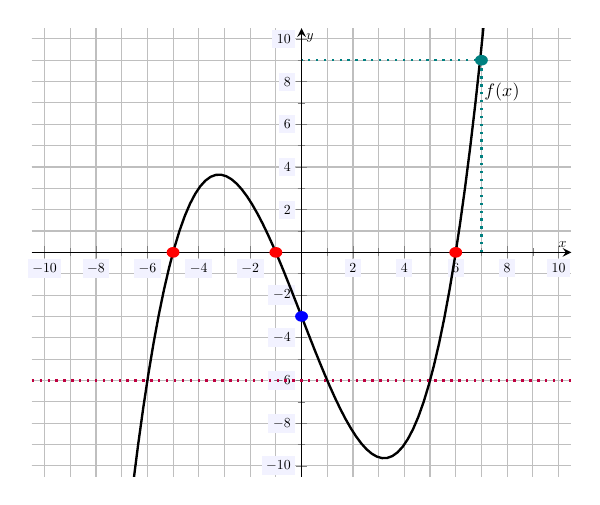
\begin{tikzpicture}[scale=1,every node/.style={scale=0.5}]
	\begin{axis}[
	grid=both,
	axis lines=middle,
	ticklabel style={fill=blue!5!white},
	xmin= -10.5, xmax=10.5,
	ymin= -10.5, ymax=10.5,
	xtick={-10,-8,...,10},
	ytick={-10,-8,...,10},
	minor tick = {-10,-9,...,10},
	xlabel=\(x\),ylabel=\(y\),
	]
	\node at (7.8,7.5) {\scalebox{1.3}{$f(x)$}};
	\addplot[line width= 0.03cm,samples=100,domain= -10:10] ({x},{1/10*(x+1)*(x + 5)*(x-6)});
	
	% Points/Lines
	\remove{
	\draw[draw=none,fill=red] (-5,0) circle (0.25);
	\draw[draw=none,fill=red] (-1,0) circle (0.25);
	\draw[draw=none,fill=red] (6,0) circle (0.25);
	}
	\remove{\draw[draw=none,fill=blue] (0,-3) circle (0.25);}
	\remove{
	\draw[draw=none,fill=teal] (7,9) circle (0.25);
	\draw[line width=0.03cm,dotted,teal] (7,0) -- (7,9) -- (0,9);
	}
	\remove{\draw[line width=0.03cm,dotted,purple] (-10.5,-6) -- (10.5,-6);}
	\end{axis}
	\end{tikzpicture}
	}
\end{minipage} \begin{minipage}[t]{0.5\textwidth} \vspace{0pt}
	\begin{enumerate}[(a)]
	\item Find the $x$-intercepts.
	
		\wans{$x= -5, -1, 6$}
		
	\item Find the $y$-intercepts.
	
		\wans{$y= -3$}
		
	\item What is $f(7)$?
	
		\wans{$f(7)= 9$}
	
	\item Solve the equation $f(x)= -6$.
	
		\wans{$x= -6, 1, 5$}
	\end{enumerate}
\end{minipage}

\end{document}